\subsection{Study selection}
Screening identified controlled trials of MDMA, LSD, psilocybin, and ayahuasca that reported harmonized AE outcomes. Reasons for exclusion most commonly included uncontrolled designs and inadequate AE reporting. The final dataset comprised session- and, when available, follow-up assessments aligned to the prespecified reference-arm policy.

\subsection{Study characteristics}
Included trials spanned a wide range of doses and assessment windows. Session-level analyses were available for all four molecules, whereas follow-up contrasts were primarily reported for LSD and MDMA. Arm-level contributions to the synthesis are summarised in \Cref{tab:study-characteristics}.

\subsection{Primary synthesis of adverse events}
Random-effects pooling across molecules showed consistent elevation of AE risk relative to the designated reference arms, as illustrated by the combined forest plot in \Cref{fig:overall-forest}. Molecule-specific significance patterns and window-specific summaries are reported in \Cref{tab:cmp_topline}. Across session analyses, LSD, MDMA, and psilocybin each yielded statistically significant overall effects, whereas follow-up models were more sparsely populated and rarely reached significance.

\IfFileExists{figures/forest_combined_all_molecules.pdf}{%
  \begin{figure}[ht]
    \centering
    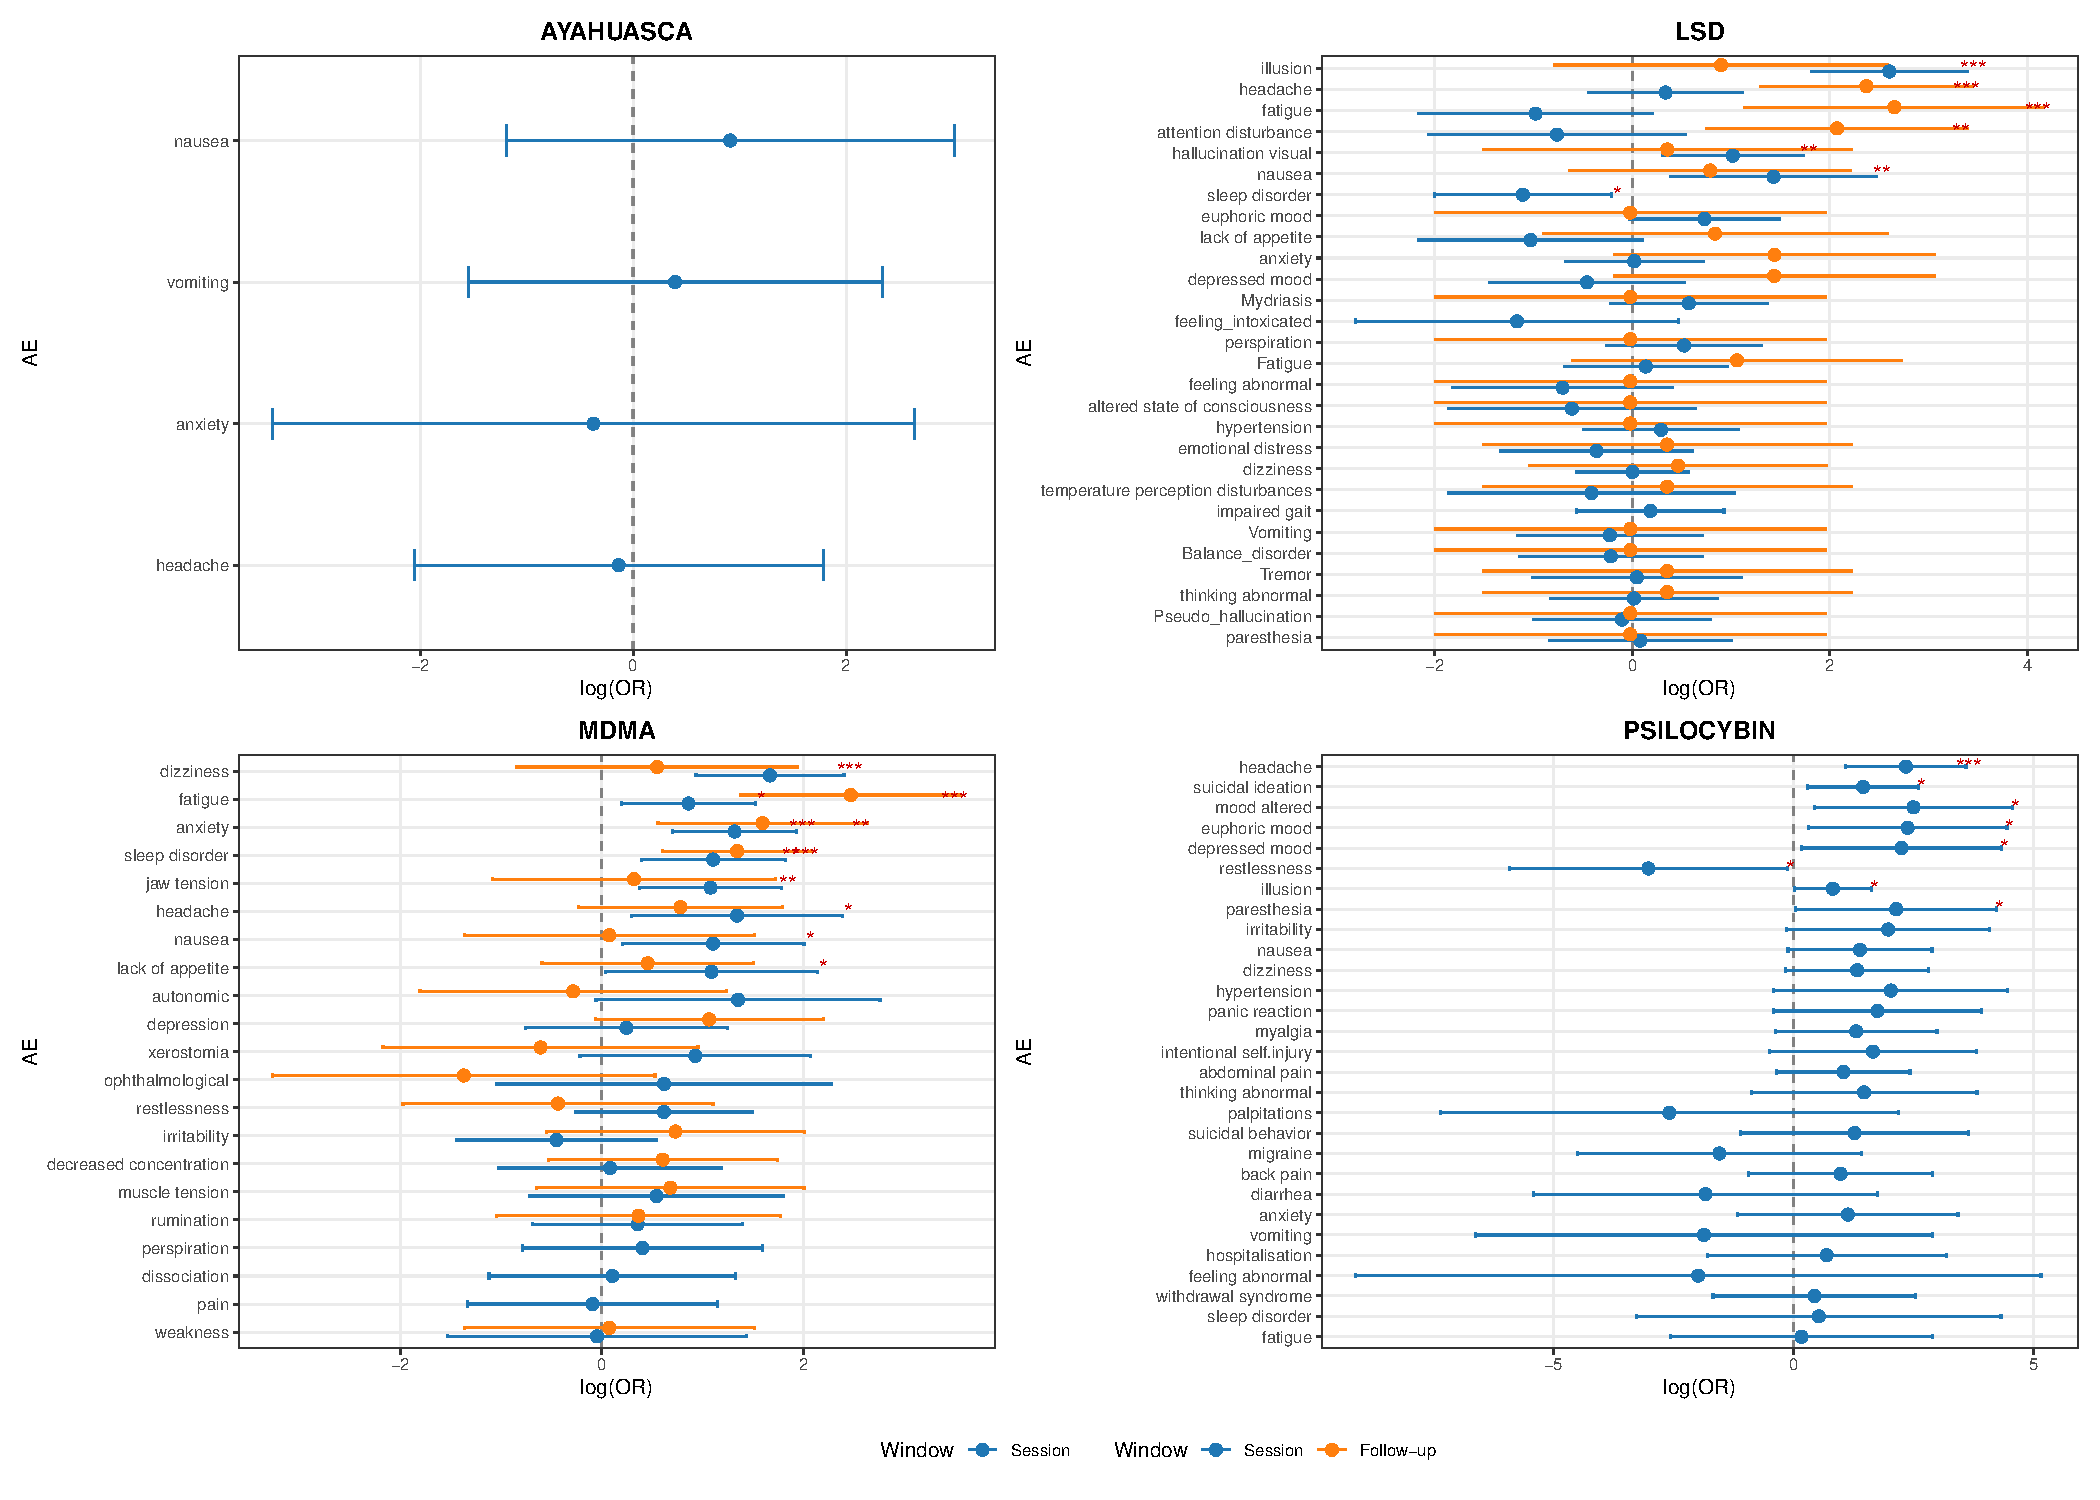
\includegraphics[width=\linewidth]{figures/forest_combined_all_molecules.pdf}
    \caption{Random-effects forest plot summarising pooled AE risk ratios across molecules and time windows.}
    \label{fig:overall-forest}
  \end{figure}
}{}

\IfFileExists{../results_compare/tables/compare_topline_publication.tex}{\begin{table}[ht]
\centering
\caption{Overall significance by molecule (session vs follow-up) and number of significant AE.}
\label{tab:cmp_topline}
\begin{tabular}{lllll}
\toprule
Molecule & Overall (session) & Overall (follow-up) & # significant AE (session) & # significant AE (follow-up) \\
\midrule
LSD & p=0.00084 *** & p=0.00235 ** & 2 &  0 \\
MDMA & p=1.47e-13 *** & p=0.0565  & 2 &  0 \\
Psilocybin & p=3.94e-11 *** &  & 1 &  \\
\bottomrule
\end{tabular}
\end{table}

}{}

\subsection{Per-adverse-event findings}
Harmonized per-AE models indicated that only a subset of AE terms demonstrated clear dose-related elevations. Significant session-level findings predominantly involved autonomic and gastrointestinal symptoms for MDMA, nausea and headache for LSD, and fatigue and hypertension for psilocybin, with corresponding $p$-values documented in \Cref{tab:cmp_ae_molecule}. Overlay plots in \Cref{fig:per-ae-overlays} show the alignment of spline-based dose--response curves across molecules for shared AE terms.

\IfFileExists{figures/master_dr_by_ae-session.pdf}{%
  \begin{figure}[ht]
    \centering
    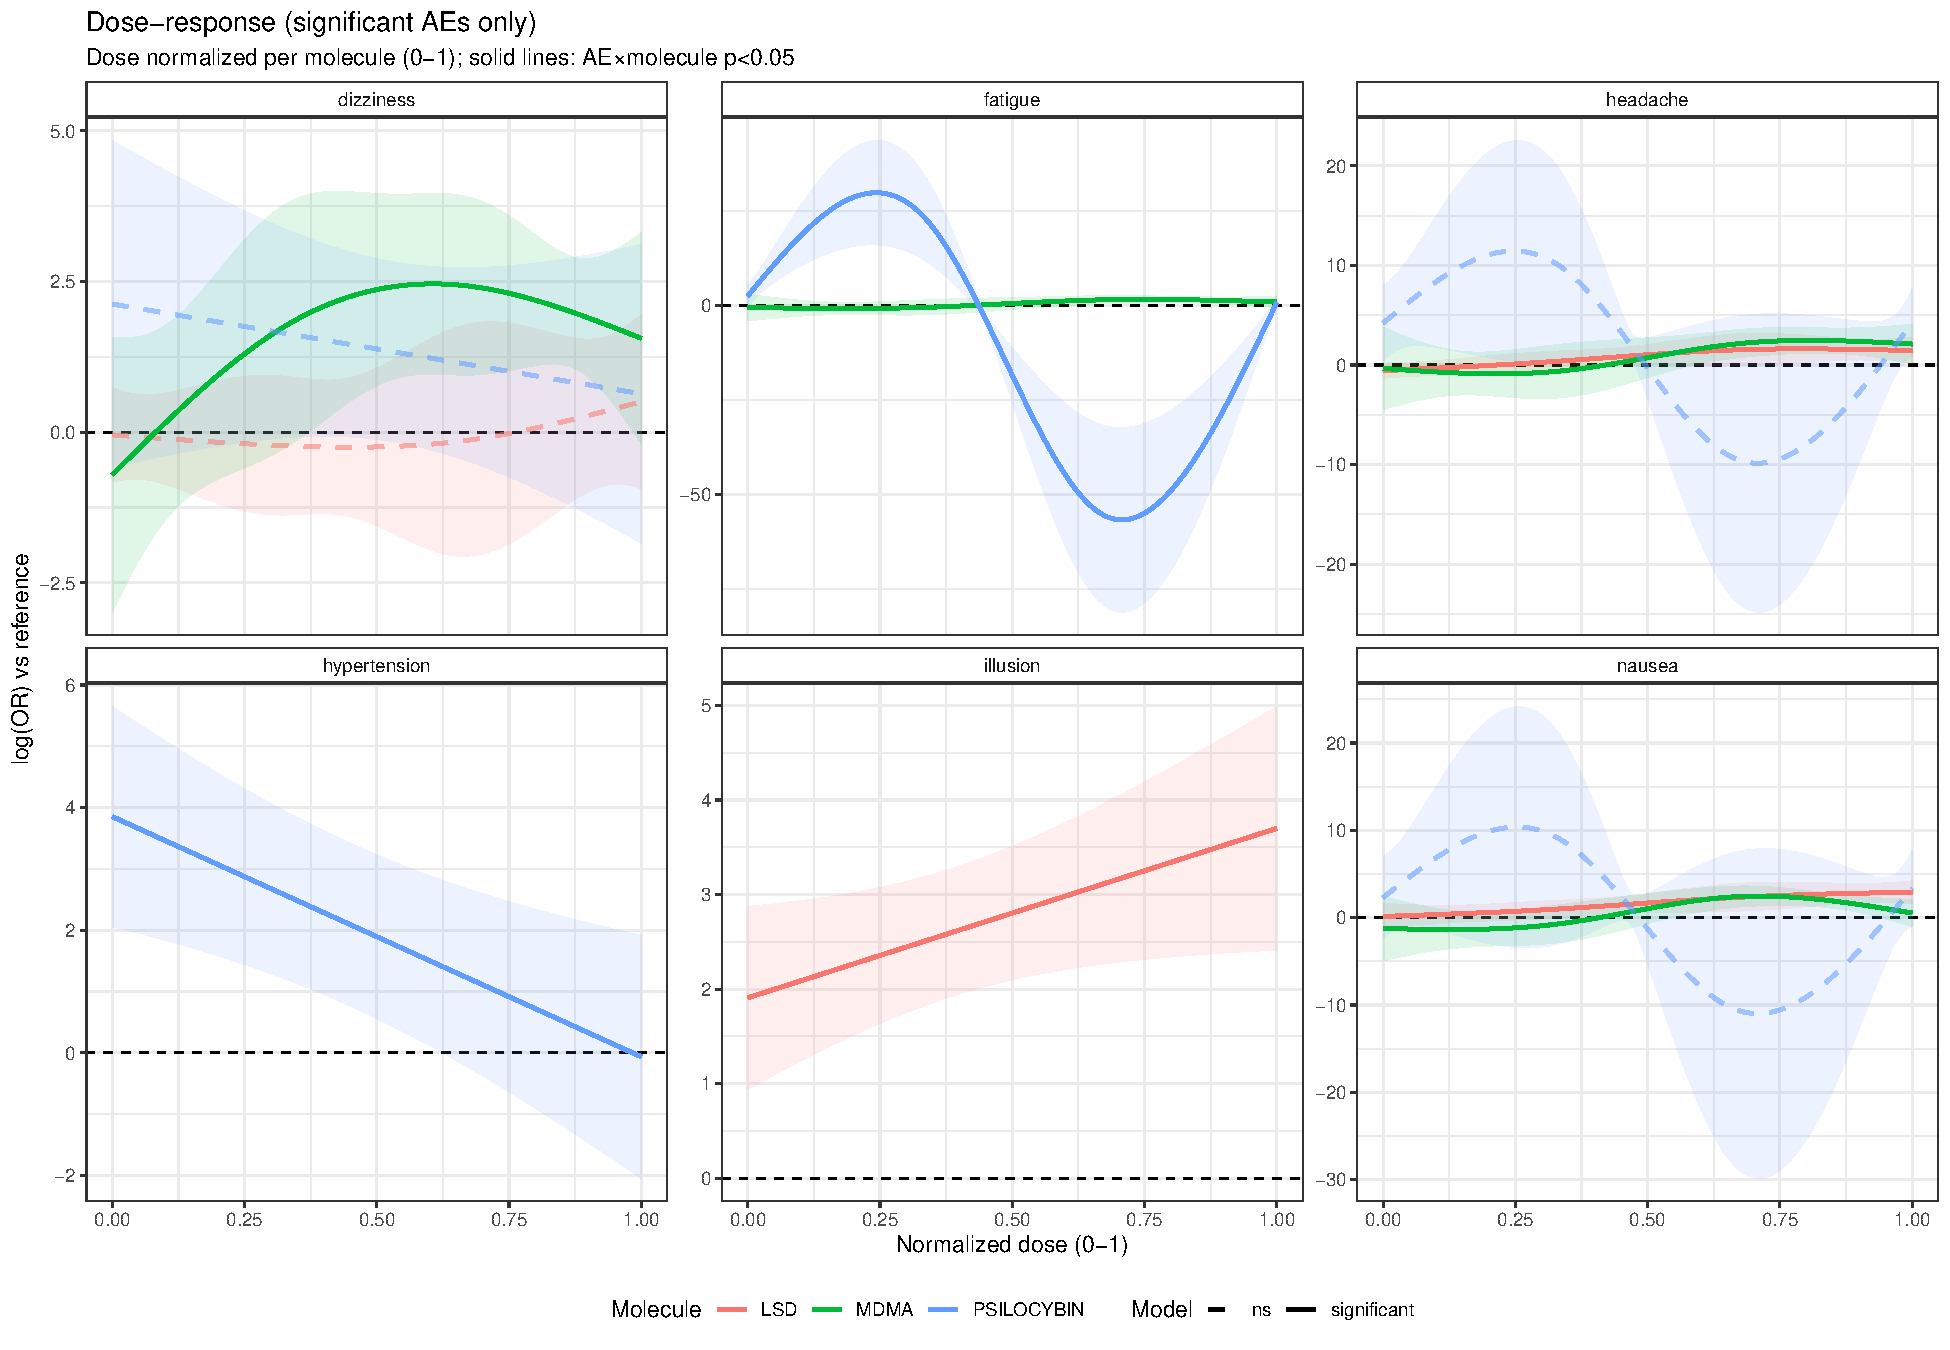
\includegraphics[width=\linewidth]{figures/master_dr_by_ae-session.pdf}
    \caption{Session-level dose--response overlays for harmonized AE terms observed across multiple molecules.}
    \label{fig:per-ae-overlays}
  \end{figure}
}{}

\IfFileExists{../results_compare/tables/compare_by_ae_molecule.tex}{\begin{table}[ht]
\centering
\caption{Per-AE comparison by molecule: session vs follow-up p-values.}
\label{tab:cmp_ae_molecule}
\begin{tabular}{llll}
\toprule
molecule & ae_term & session & follow \\
\midrule
LSD & anxiety & p=0.713  &  \\
LSD & attention disturbance & p=0.526  & p=0.15  \\
LSD & dizziness & p=0.89  & p=0.912  \\
LSD & emotional distress & p=0.256  &  \\
LSD & feeling abnormal & p=0.372  &  \\
LSD & headache & p=0.0104 * & p=0.629  \\
LSD & nausea & p=0.025 * & p=0.885  \\
LSD & perspiration & p=0.511  &  \\
LSD & temperature perception disturbances & p=0.774  &  \\
LSD & thinking abnormal & p=0.662  &  \\
MDMA & anxiety & p=0.0724  &  \\
MDMA & autonomic & p=0.0719  &  \\
MDMA & depression & p=0.0456 * &  \\
MDMA & dissociation & p=0.362  &  \\
MDMA & dizziness & p=0.147  &  \\
MDMA & fatigue & p=0.159  &  \\
MDMA & headache & p=0.00654 ** &  \\
MDMA & irritability & p=0.284  &  \\
MDMA & jaw tension & p=0.491  &  \\
MDMA & lack of appetite & p=0.156  &  \\
MDMA & muscle tension & p=0.509  &  \\
MDMA & nausea & p=0.336  &  \\
MDMA & ophthalmological & p=0.196  &  \\
MDMA & pain & p=0.129  &  \\
MDMA & perspiration & p=0.072  &  \\
MDMA & restlessness & p=0.374  &  \\
MDMA & rumination & p=0.709  &  \\
MDMA & sleep disorder & p=0.0643  & p=0.539  \\
MDMA & xerostomia & p=0.836  &  \\
Psilocybin & abdominal pain & p=0.502  &  \\
Psilocybin & anxiety & p=0.591  &  \\
Psilocybin & fatigue & p=2.54e-06 *** &  \\
Psilocybin & headache & p=0.207  &  \\
Psilocybin & nausea & p=0.537  &  \\
Psilocybin & suicidal ideation & p=0.462  &  \\
\bottomrule
\end{tabular}
\end{table}

}{}

\subsection{Dose--response relationships}
Dose--response meta-regression demonstrated molecule-specific trajectories (\Cref{fig:dose-response}). MDMA exhibited approximately monotonic increases in AE risk with higher doses, whereas LSD and psilocybin presented non-linear patterns consistent with restricted cubic spline fits. Ayahuasca contributed a single-dose contrast and was therefore not modeled for continuous dose effects.

\IfFileExists{figures/master_dr_by_molecule-session.pdf}{%
  \begin{figure}[ht]
    \centering
    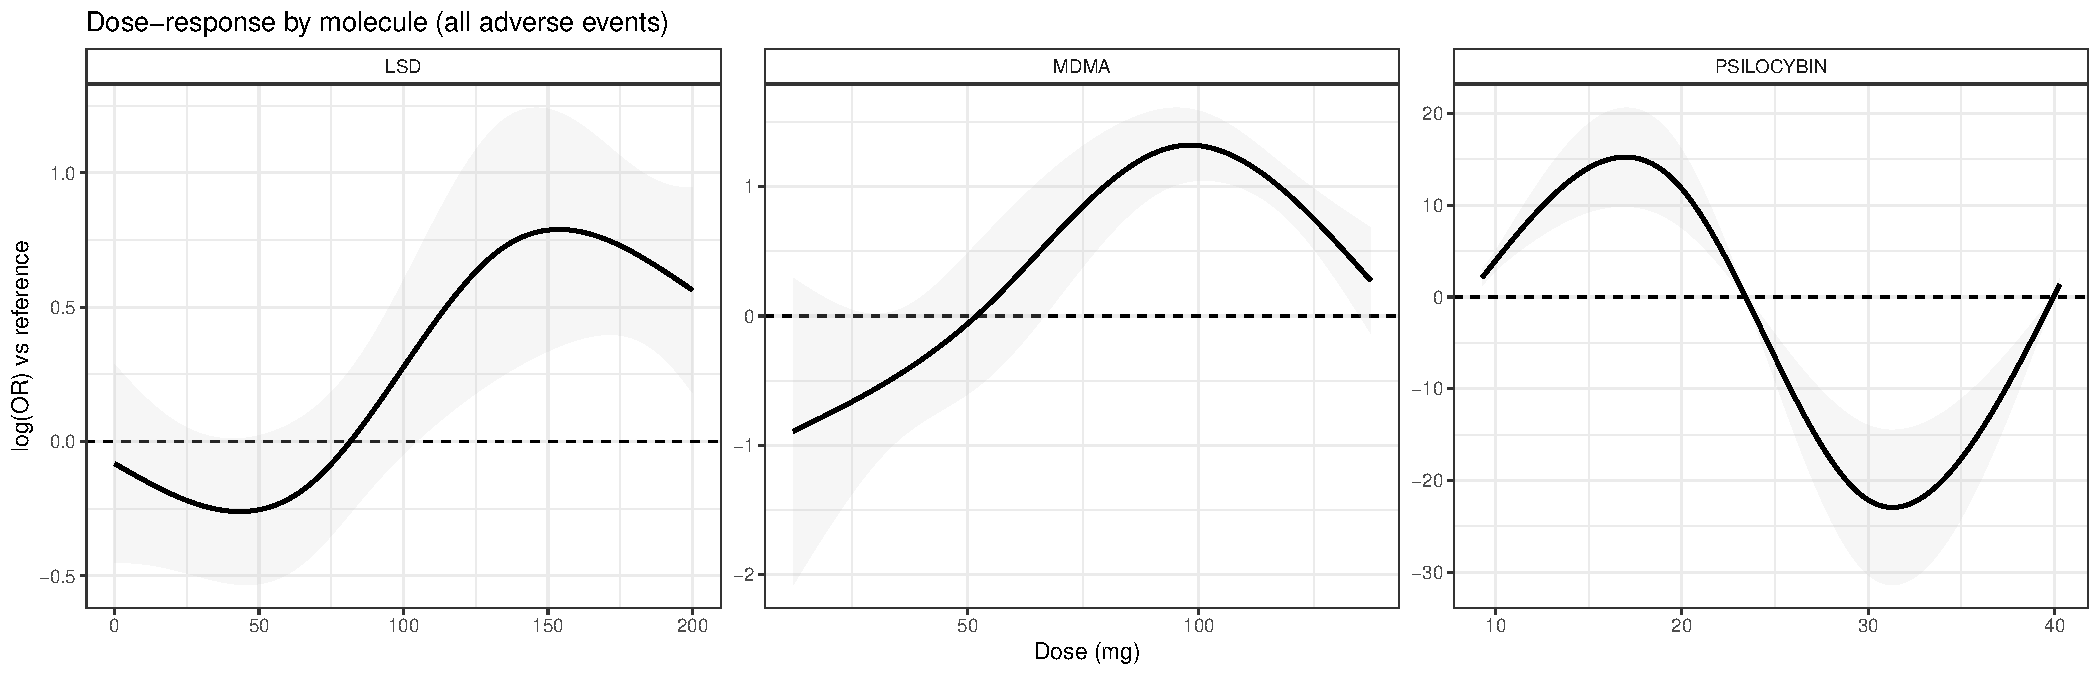
\includegraphics[width=\linewidth]{figures/master_dr_by_molecule-session.pdf}
    \caption{Session-level dose--response curves derived from spline meta-regressions for each molecule.}
    \label{fig:dose-response}
  \end{figure}
}{}

\subsection{Session versus follow-up comparisons}
Comparative analyses of session and follow-up windows highlighted attenuation of effects at later assessments, as visualised in \Cref{fig:session-followup}. Table-based contrasts (\Cref{tab:cmp_topline,tab:cmp_ae_molecule}) show that several AE terms with session-level significance did not retain statistical support at follow-up, reflecting limited sample sizes and fewer reported contrasts.

\IfFileExists{figures/dr_session_vs_followup.pdf}{%
  \begin{figure}[ht]
    \centering
    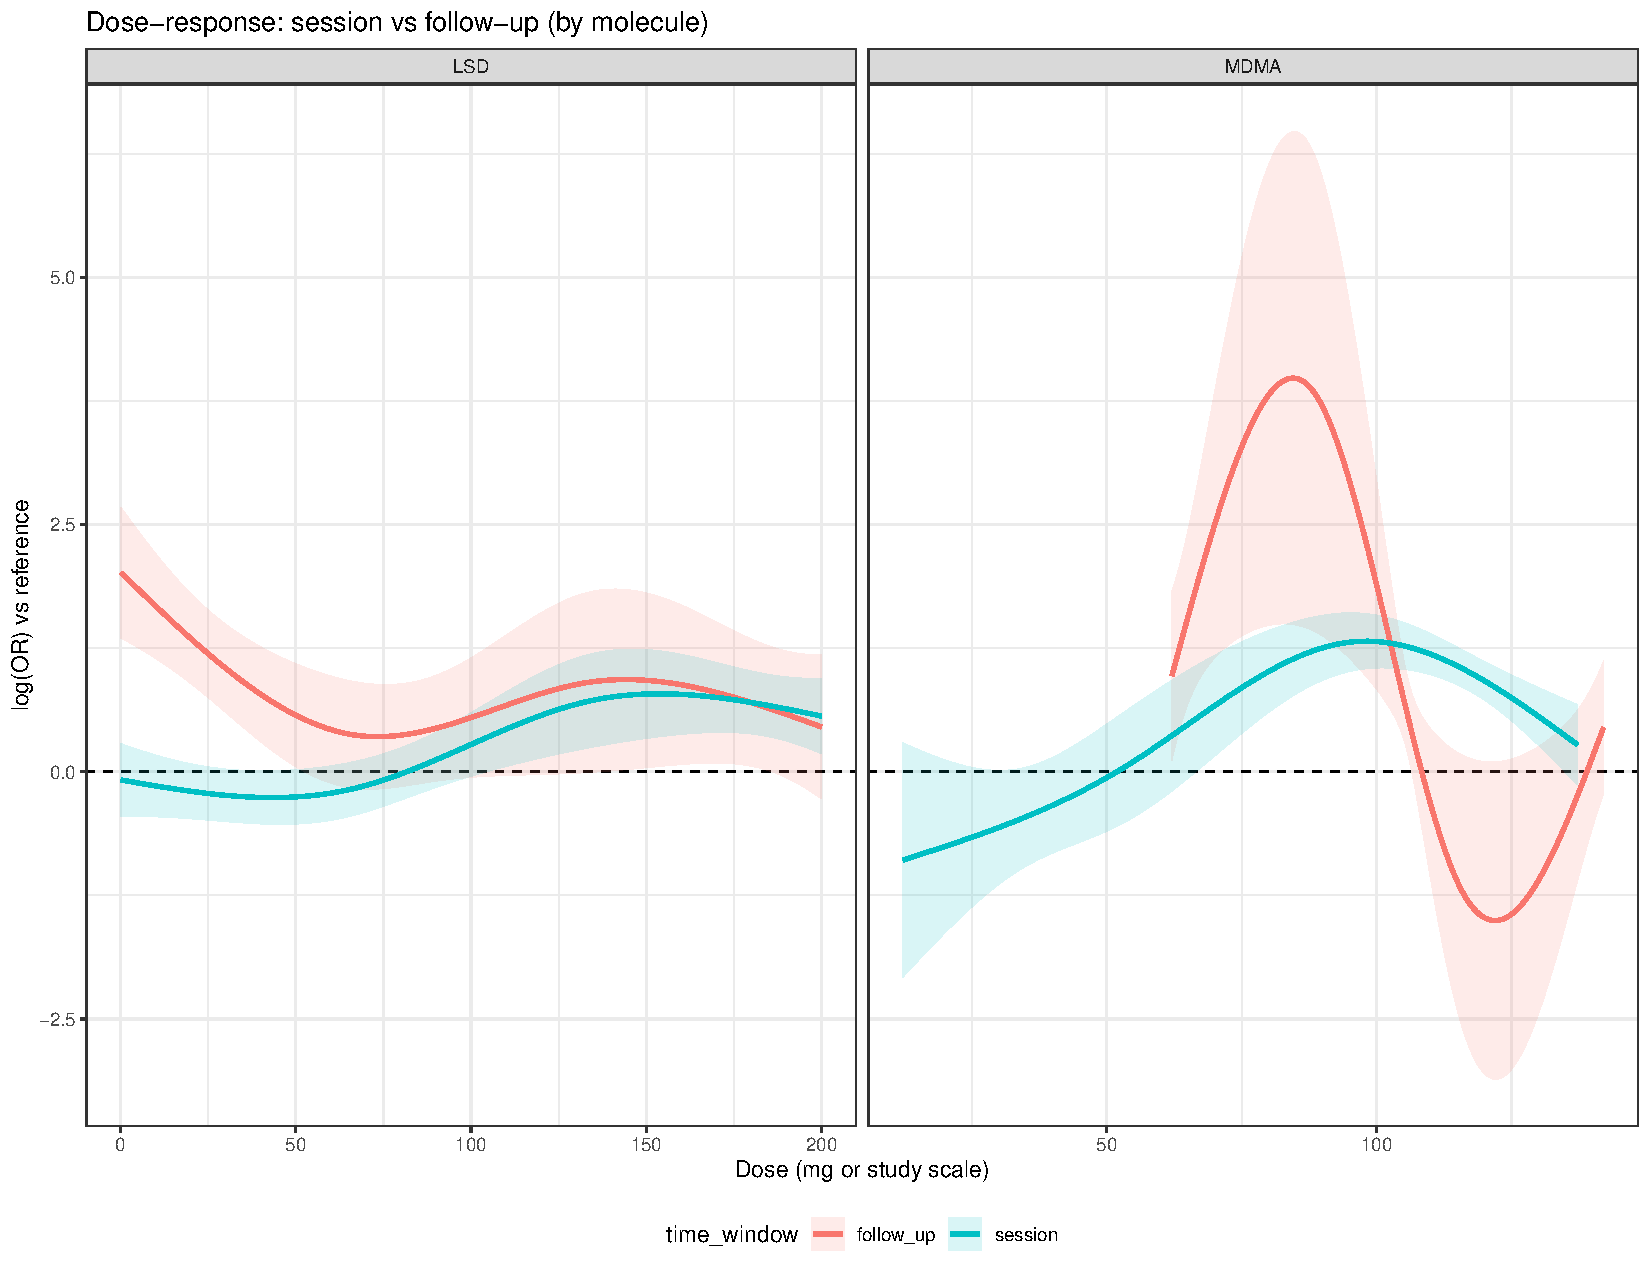
\includegraphics[width=\linewidth]{figures/dr_session_vs_followup.pdf}
    \caption{Comparison of session and follow-up dose--response slopes across molecules.}
    \label{fig:session-followup}
  \end{figure}
}{}
